\usetikzlibrary {3d}
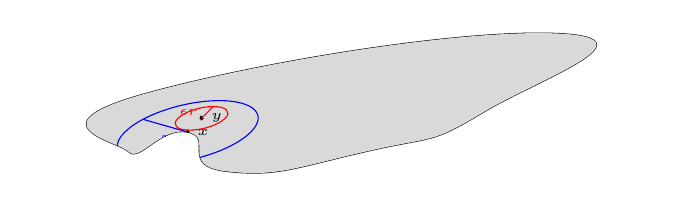
\begin{tikzpicture}
  \begin{scope}[x={(1cm,0cm)}, y={(0.5cm,0.5cm)}, z={(0cm,1cm)}]
      % Draw the reference region (smooth cycle) and fill it with gray
      \draw plot [smooth cycle, tension=1] coordinates {(-.5,1.5)(0,0)(.5,.5)(1.5,-.5)(3,0)(4,1)(4,3)};
      \fill[gray!30] plot [smooth cycle, tension=1] coordinates {(-.5,1.5)(0,0)(.5,.5)(1.5,-.5)(3,0)(4,1)(4,3)};
      
      % Clip the drawing to the region inside the smooth cycle
      \clip plot [smooth cycle, tension=1] coordinates {(-.5,1.5)(0,0)(.5,.5)(1.5,-.5)(3,0)(4,1)(4,3)};
      
      % Draw the blue circle only inside the clipped region
      \node (p1) at (0.5, 0.5) {$\cdot$};
      \draw[blue] (p1) circle[x radius=.8, y radius=.8];
      \draw[fill=black](0.5,0.5) circle (.5 pt) node [right] {\tiny $x$};
      \draw[blue](0.5,0.5) -- (-.22,.82) node [midway,below] {\tiny $r$};
      
              
      % Draw the red circle only inside the clipped region
      \node (p2) at (0.5, 0.85) {$\cdot$};
       \draw[fill=black](0.5,0.85) circle (.5 pt) node [right] {\tiny $y$};
      \draw[red] (p2) circle[x radius=.3, y radius=.3];
      \draw[red](0.5,0.85) -- (.5,1.15) node [midway,left] {\tiny $\epsilon r$};
  \end{scope}
\end{tikzpicture}